\documentclass{article}

\usepackage{arxiv}

\usepackage[utf8]{inputenc} % allow utf-8 input
\usepackage[T1]{fontenc}    % use 8-bit T1 fonts
\usepackage{hyperref}       % hyperlinks
\usepackage{url}            % simple URL typesetting
\usepackage{booktabs}       % professional-quality tables
\usepackage{amsfonts}       % blackboard math symbols
\usepackage{microtype}      % microtypography
\usepackage{graphicx}
\usepackage{natbib}
\usepackage{doi}
\usepackage{listings}
\usepackage{lineno}
\usepackage{setspace}

\linenumbers

\title{Enabling high resolution hydrologic routing with machine learning assisted waterbody classification}

%\date{September 9, 1985}	% Here you can change the date presented in the paper title
\date{} 					% Or removing it

\author{
	\href{https://orcid.org/0000-0002-5924-2464}{
\includegraphics[scale=0.06]{orcid.pdf}\hspace{1mm}Jemma Stachelek},
	\href{https://orcid.org/0000-0001-6052-199X}{
\includegraphics[scale=0.06]{orcid.pdf}\hspace{1mm}
	 Charles J. Abolt},
	\href{https://orcid.org/0000-0001-5803-9686}{
\includegraphics[scale=0.06]{orcid.pdf}\hspace{1mm}
	 Jon Schwenk} \\
	Earth and Environmental Sciences\\
	Los Alamos National Laboratory\\
	Los Alamos, NM, USA, 87544 \\
	\texttt{jsta@lanl.gov} \\
}

% Uncomment to remove the date
%\date{}

% Uncomment to override  the `A preprint' in the header
\renewcommand{\headeright}{\href{https://doi.org/}{DOI: 10.000/XXXXX}}
\renewcommand{\undertitle}{This is a draft of a Manuscript in preparation for publication in Geophysical Research Letters \href{https://doi.org/10.1000/XXXXX}{DOI: 10.1000/XXXXX}}
\renewcommand{\shorttitle}{ML assisted waterbody classification for routing}

%%% Add PDF metadata to help others organize their library
%%% Once the PDF is generated, you can check the metadata with
%%% $ pdfinfo template.pdf
\hypersetup{
pdftitle={Enabling high resolution hydrologic routing with machine learning assisted waterbody classification},
pdfsubject={stat.AP},
pdfauthor={Jemma Stachelek}
}

\begin{document}
\maketitle
\doublespacing

\vspace{-2em}
\section*{Keypoints}
\begin{enumerate}
	\item We demonstrate a deep learning pipeline for waterbody database creation with a novel waterbody classifier approaching 80\% accuracy
	\item It produced similar results in terms of waterbody count, surface area, and types as a much more expensive to produce hand-curated product
	\item The modular design of the pipeline is future-proof to forthcoming data products and is easily tailored to specific hydrologic routing tasks
\end{enumerate}
\newpage

\section*{Abstract}	
	Some waterbody databases are focused on delineating all areas of standing water irrespective of the persistence or “type” of the waterbody. However, for other applications, such as integration of waterbodies into hydrologic routing schemes, capturing the long-term dynamics of persistent waterbodies is of critical importance. The creation of such databases is costly, often requiring manual intervention in many of the underlying steps. As an alternative, we developed a machine learning pipeline that facilitates the rapid, accurate, and inexpensive creation of these databases using deep neural networks operating on high resolution imagery. In addition to basic delineation tasks, capturing time dynamics, and detection of waterbody boundaries, the pipeline includes a novel approach to classify and prune spurious and ephemeral non-lake waterbodies. We demonstrate the accuracy, performance, and consistency of the pipeline compared with a much more expensive to produce hand-curated product with the aim of scaling to continental and global extents.

\section*{Plain Language Summary}
	Detailed simulations of streamflow routing require a database of lakes and other waterbodies which are persistent in time.  The construction of these persistent waterbody databases typically requires significant labor and computational expense. One step that has remained resistant to automation is that of pruning ephemeral and/or spurious waterbodies. As a solution to this challenge, we developed a deep learning classifier model as part of an end-to-end database production pipeline. We demonstrate the accuracy, performance, scaling, and consistency of the pipeline compared with a much more expensive to produce hand-curated product. The modular design of the pipeline makes it future-proof to the development of new water detection, waterbody delineation, and classification products/methodologies as well as easily tailored to a variety of hydrologic routing tasks.

\section{Introduction}
The uses of waterbody databases and the motivations for their creation are varied. Some waterbody databases are focused on delineating all areas of standing water irrespective of the persistence or “type” of the waterbody. This can be valuable for quantifying the state of the system with respect to general wetness, deriving estimates of greenhouse gas flux, or  characterizing the changing seasonality of a system \citep{cooleyArcticBorealLake2019, mullenUsingHighResolution2023}. However, for other applications, such as integration of waterbodies into hydrologic routing schemes, capturing the long-term dynamics and extent of persistent waterbodies is of critical importance \citep{davidDecadeRAPIDReflections2016,mizukamiVectorBasedRiver2021}. The construction of these persistent waterbody databases typically requires significant labor and computational expense for steps like manual tracing of waterbody outlines and automated correction of missing data \citep{amatulliHydrography90mNewHighresolution2022,lehnerGlobalRiverHydrography2013}.

Although these labor-intensive activities have been the subject of prior waterbody delineation/detection algorithm development efforts \citep{khandelwal2022realsat}, one step that remains as an unaddressed manual labor cost, is that of pruning ephemeral and/or spurious waterbodies (hereafter referred to simply as “spurious waterbodies”) from datasets prior to use in hydrologic routing. These spurious waterbodies can include all or some of the following entities depending on the specific needs of the hydrologic routing scheme being implemented: run-of-the-river embayments, flooded agricultural fields, river segments, and coastal lagoons. Identifying and removing these waterbodies is challenging both because of the limited accuracy of delineation algorithms for specific regions/ecotypes and because imagery archives may lack the context of repeat observations necessary for tracking individual waterbodies through time relative to the emergence of climate signals \citep{hawkinsTimeEmergenceClimate2012,khandelwal2022realsat}. 

For example, at high latitudes, earth observation satellites have a limited ability to collect imagery in polar winter (notwithstanding the fact that they are frozen) resulting in a lessened ability to recover the dynamic condition of waterbodies of interest \citep{musterPeRLCircumArcticPermafrost2017,pekelHighresolutionMappingGlobal2016}. In river-adjacent floodplains, the morphological similarities between floodplain lakes and the rivers themselves can lead to high rates of spurious non-lake waterbodies being entered into the database \citep{piMappingGlobalLake2022}. Beyond lack of observations in specific regions and morphologic disambiguation difficulties in specific ecotypes, some imagery archives, especially those containing recently collected high-resolution images, may lack a sufficiently long observational period-of-record to encompass the full range of hydrologic conditions experienced at the given location \citep{wulderCurrentStatusLandsat2019}. Taken together, these challenges mean that critical parts of persistent waterbody database production remain largely manual despite the wider availability of high(er) resolution imagery and the development of advanced machine learning (ML) algorithms.

As a potential solution, we built a multi-stage ML pipeline that not only identifies persistent waterbodies while capturing time dynamics and detecting waterbody edges at high resolution, but also includes an automated waterbody classifier such that users can exclude specific waterbody types. In the first stage, a “raw” set of waterbodies in each time step are identified. In the second stage, this raw set of waterbodies is pruned based on an ML classifier into only the desired types of waterbodies (i.e. only lakes, lakes and flooded fields, etc). In the final stage, waterbodies across time steps are consolidated such that those which are disparate in one time step are assigned identical “recurrence” identifiers if they are joined or overlapping in any of the other time steps in the period of record. Users are able to set a threshold that determines what fraction of the period of record is required for a waterbody to be deemed persistent enough to remain in the pipeline. In this way, users are able to adjust the lumping and splitting as appropriate for their intended application while maintaining the hydrologic history of the waterbody and accounting for splitting/reforming as a result of flooding and/or drying. A critical design feature that cuts across all the stages of our pipeline is that of modularity. We've made it easy for users to substitute alternative data products and algorithms for any step of the pipeline based on their needs and the specific downstream application of interest. As a result, our pipeline is future-proof to the development of forthcoming models or state-of-the-art data products. Should a research team develop or release a new state-of-the-art product (e.g. \citet{mullenUsingHighResolution2023}), it can easily be incorporated.

We demonstrate our pipeline in a case study set in the Yukon Flats watershed in Alaska, USA. For our pipeline, we use a deep convolutional neural network operating on high resolution (3-5m) Planet imagery for surface water detection feeding into a neural network classifier for waterbody type identification. For the training of the neural network classifier, we define a waterbody database as a collection of persistent, well-defined areas of standing water excluding ephemeral waterbodies such as temporary agricultural ponds and making no distinction between reservoirs and “natural” lakes, which may or may not be managed (see Methods section for detailed definitions and thresholds). We show that pipeline output is consistent with much more expensive to produce hand-curated products and that it enables automated waterbody detection, classification and change detection, while keeping labor costs and computational overhead low. 


\section{Methods}

\subsection{Pipeline Overview}

Our Python-based pipeline for waterbody delineation, classification, and change detection starts with a user providing a preexisting area-of-interest (AOI) GeoTiff “basemap” or vector bounding box to our wbextractor tool (zenodo DOI). This AOI, together with a user-defined project folder to hold tool output, and (if desired) a classification model “checkpoint”, is all that is necessary to execute the pipeline (Figure 1). The wbextractor tool then uses the AOI bounds to create an imagery catalog via one of several web API services. The examples shown hereafter and throughout our case study use the Planet Python client to query the Planet imagery API (https://developers.planet.com/docs/apis/, which requires payment or a non-commercial exemption such as through the NASA Commercial Smallsat Data Acquisition Program, CSDA). After wbextractor creates a catalog, downloads each image to a user-specified project folder, and subjects each to a suite of quality checks, they are passed to the DeepWaterMap machine learning tool for water segmentation \citep{isikdogan2019seeing}. We used the publicly available DeepWaterMap (DWM) convolutional neural network checkpoint, which was trained on Landsat imagery, to delineate areas of surface water. We modified DeepWaterMap to process imagery with fewer bands than Landsat (e.g. Planet). Users seeking to use DeepWaterMap with imagery having different numbers of bands or bands in a different order than the training data would need to similarly modify the DWM source code. Following segmentation, we implemented a connected components routine using the scikit-image library \citep{vanderwalt2014} to identify a raw set of candidate waterbodies.

\begin{figure}
	\centering
	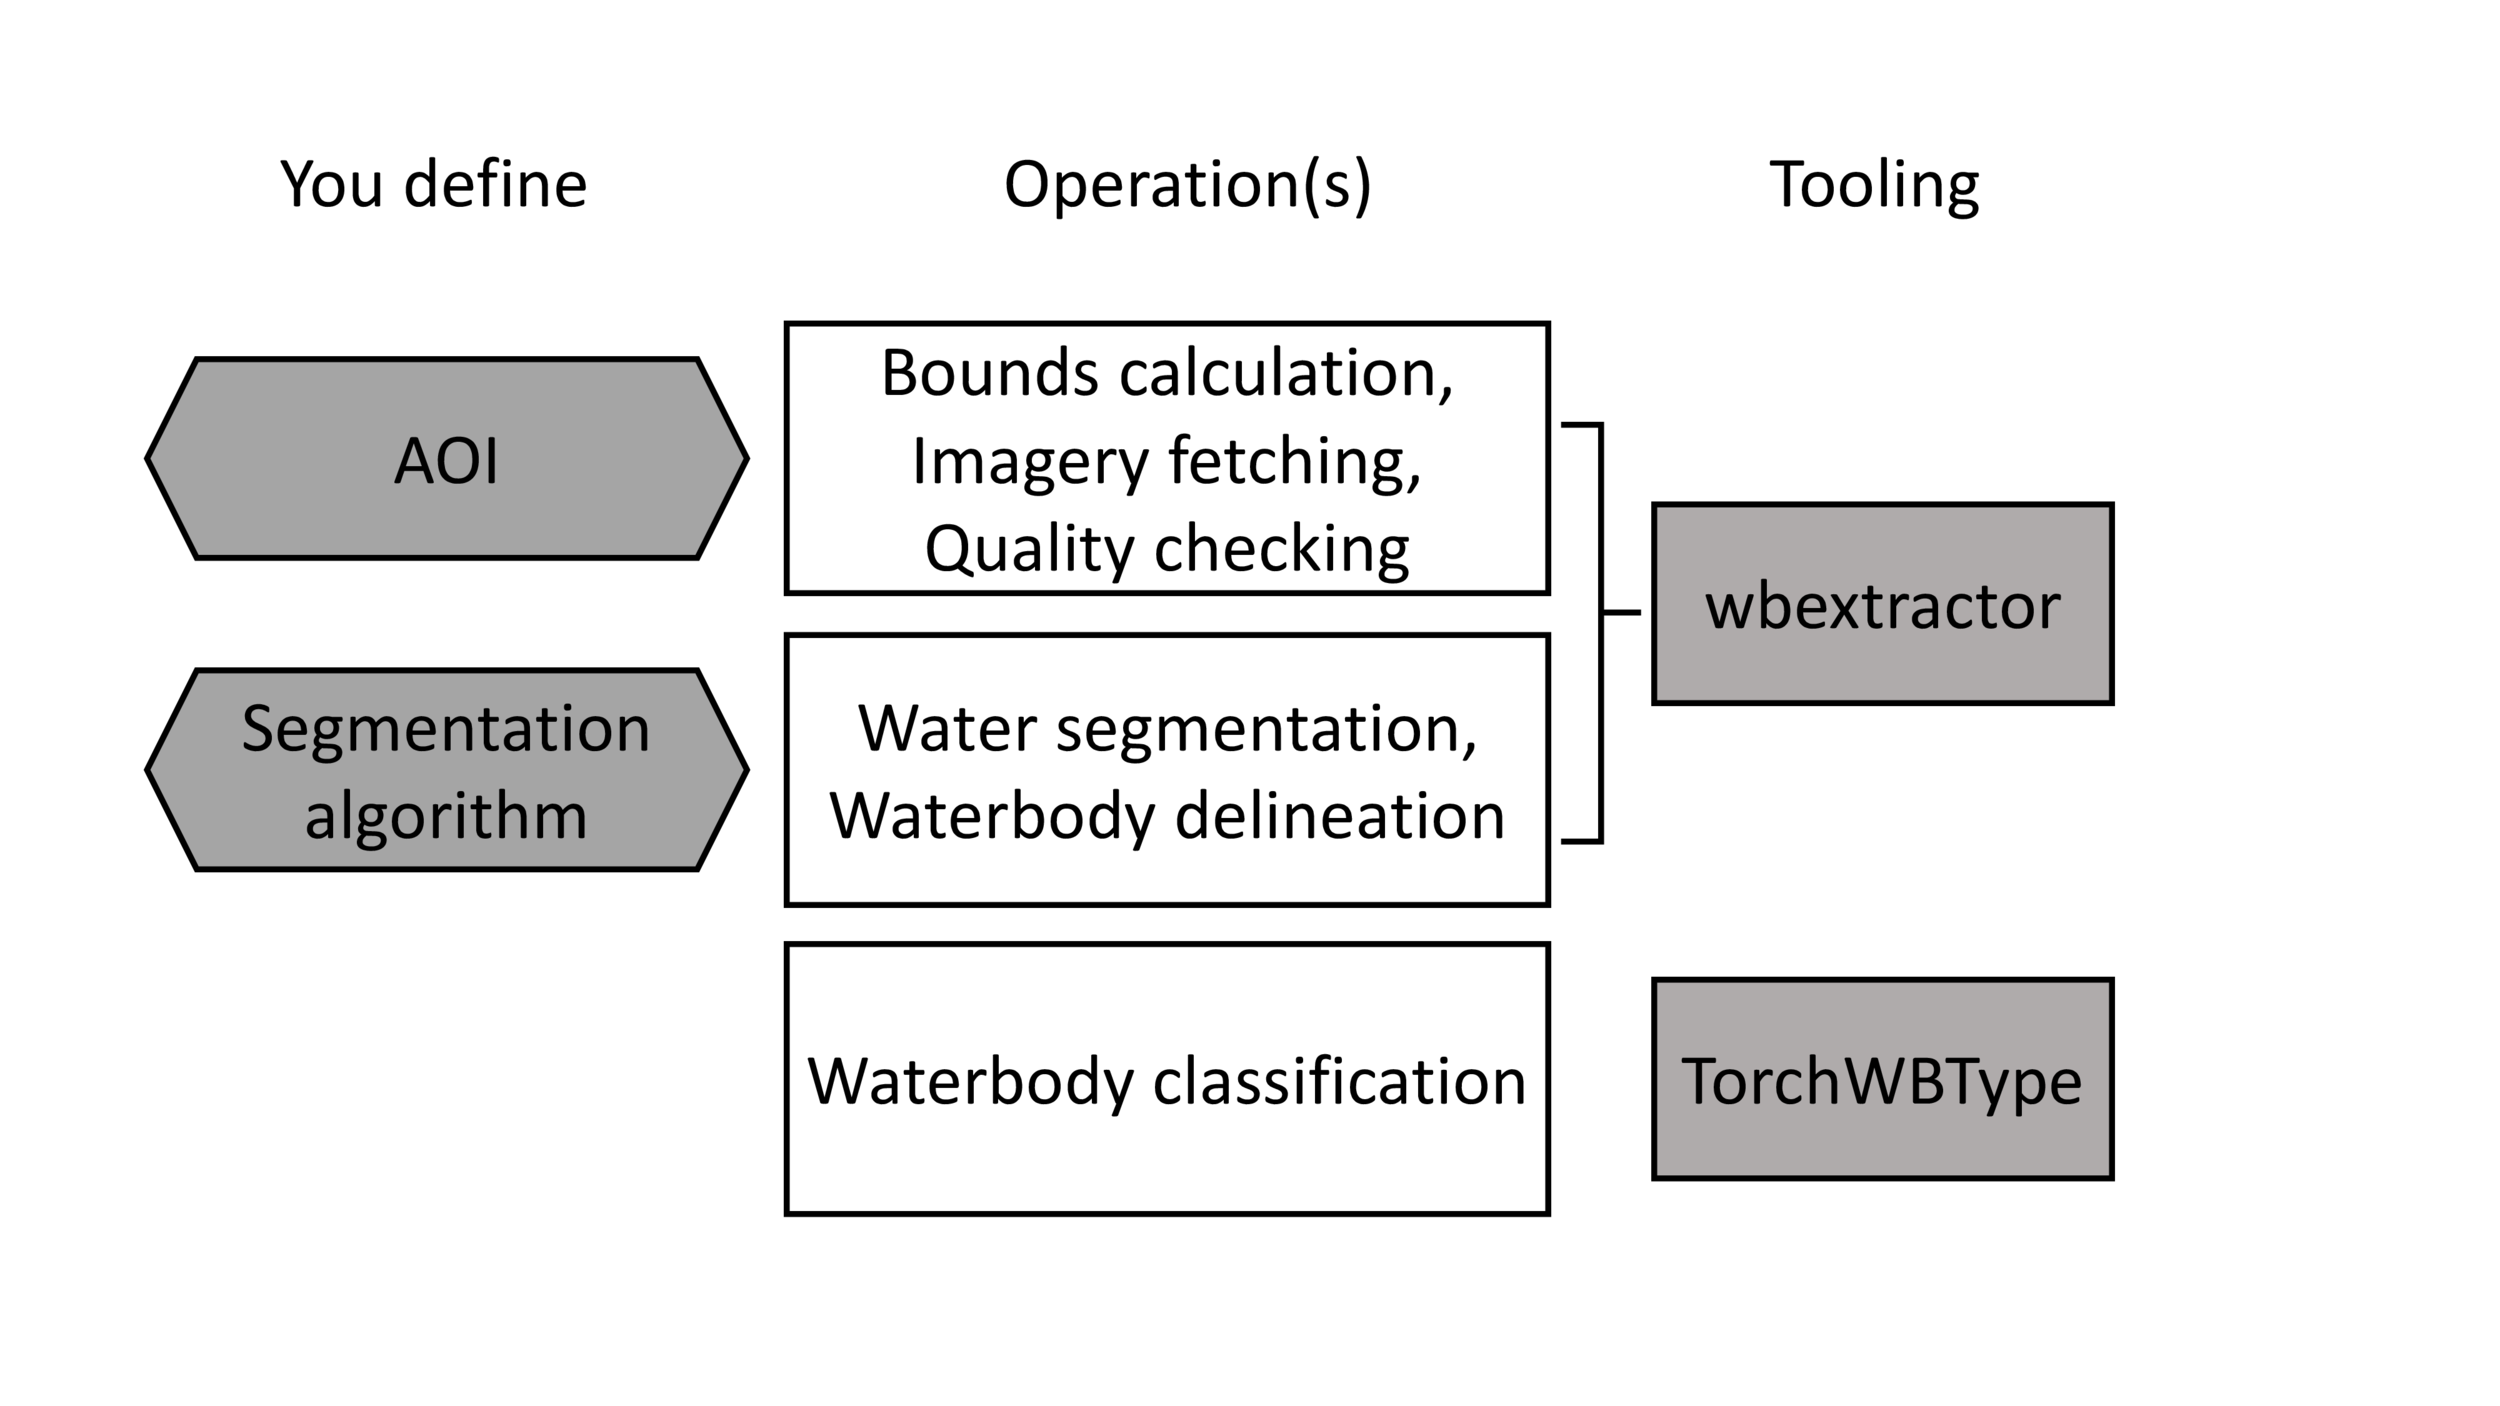
\includegraphics[width=11cm]{../figures/diagram_pipeline}
	\caption{Diagram of our waterbody delineation, classification, and change detection pipeline. Filled rectangles denote software tools for delineating (wbextractor) and classifying (TorchWBType) waterbodies. Each software tool is linked to the operations they provide by solid (wbextractor) and dashed (TorchWBType) lines.}
	\label{fig:diagram_pipeline}
\end{figure}

\subsection{TorchWBType Description}

Next, we developed an ML tool called TorchWBType to identify persistent waterbodies and determine whether or not a given polygon should be classified as a lake (Zenodo DOI). This neural network based classifier provides a method for determining the relative similarity of a candidate polygon to a set of manually labeled lakes and non-lakes. It does these comparisons using a large number of input features representing polygon characteristics such as the number of polygon interiors (i.e. “holes”), polygon eccentricity, and major axis length (see Table S2 for a complete listing). When comparing a candidate polygon against a model checkpoint, TorchWBType provides not only a lake versus non-lake determination but also the associated likelihood and uncertainty as to whether it is truly a lake and not a “false positive” (e.g. a flooded agricultural field, a river segment, or a coastal lagoon). The model checkpoint, which is provided with each installation of TorchWBType, was trained on a set of georeferenced polygons (n=540) from the global ReaLSAT database \citep{khandelwal2022realsat} and was manually labeled using a React-based LeafLet dashboard. The polygons from ReaLSAT were selected at random without limitation to geographic region. The architecture of a TorchWBType model consists of a GPU-accelerated, neural network-based, binary classification model coded in PyTorch with 3 hidden layers and intermediate ReLU activation functions. TorchWBType uses the Adam optimizer with a default base learning rate of $10^{-4}$. 

Following the waterbody classification step, there is a final automated “recurrence” step whereby waterbody polygons across time steps are consolidated such that waterbodies which are disparate in one time step are assigned identical “recurrence” identifiers if they are joined in any of the other time steps in the period of record. Users are given an option to pre-determine a minimum recurrence threshold below which candidate waterbodies will be considered to be ephemeral and discarded in the final dataset. The operations in this recurrence stage are meant to incorporate the hydrologic history of a given waterbody (or set of waterbodies) to account for splitting and reforming as a result of flooding and/or drying. At the conclusion of the pipeline, users are provided with a series of waterbody outlines which are then labeled with common waterbody recurrence identifiers for post processing to identify, for example, the typical seasonal extent of a given waterbody or its maximum/mean/minimum extent.

\subsection{Case study Description}

We tested our pipeline in an area of the Yukon Flats watershed in Alaska, USA (Figure 2). We chose this area, which surrounds Beaver Creek, because it contains delineated waterbodies from a range of data sources having varying resolutions and methodologies of creation (Figure 3). These include HydroLAKES \citep{lehnerGlobalRiverHydrography2013}, GLAKES \citep{piMappingGlobalLake2022}, and PeRL \citep{musterPeRLCircumArcticPermafrost2017}. Although HydroLAKES and GLAKES are both global products, GLAKES had a much more automated construction compared to HydroLAKES while PeRL is distinct from the other datasets because it is much more limited in geographic extent than the other two products. Also, it was constructed entirely by manual delineation (mostly from aerial imagery), and has a much finer resolution (PeRL:  5-6m, HydroLAKES: 30m, GLAKES: 30m, wbextractor: 3-5m). The PeRL, HydroLAKES, GLAKES, datasets were based on imagery collected in the following time periods 2002-2013, 2000, and 1984-2019 respectively. Beyond coverage of multiple waterbody datasets, another motivation for choosing this area was that it contains a diverse set of waterbodies which are easily mis-classified by automated techniques (particularly within “context-less” bounding boxes) including small river segments, large river segments, and temporary/ephemeral lakes. We used high resolution (3-5 m) Planet imagery for the period of 2017-2022 and limited the results to images passing strict quality criteria filters requiring candidate images to have 100\% visibility, 0\% cloud cover, and 0\% snow and ice.

\begin{figure}
	\centering
	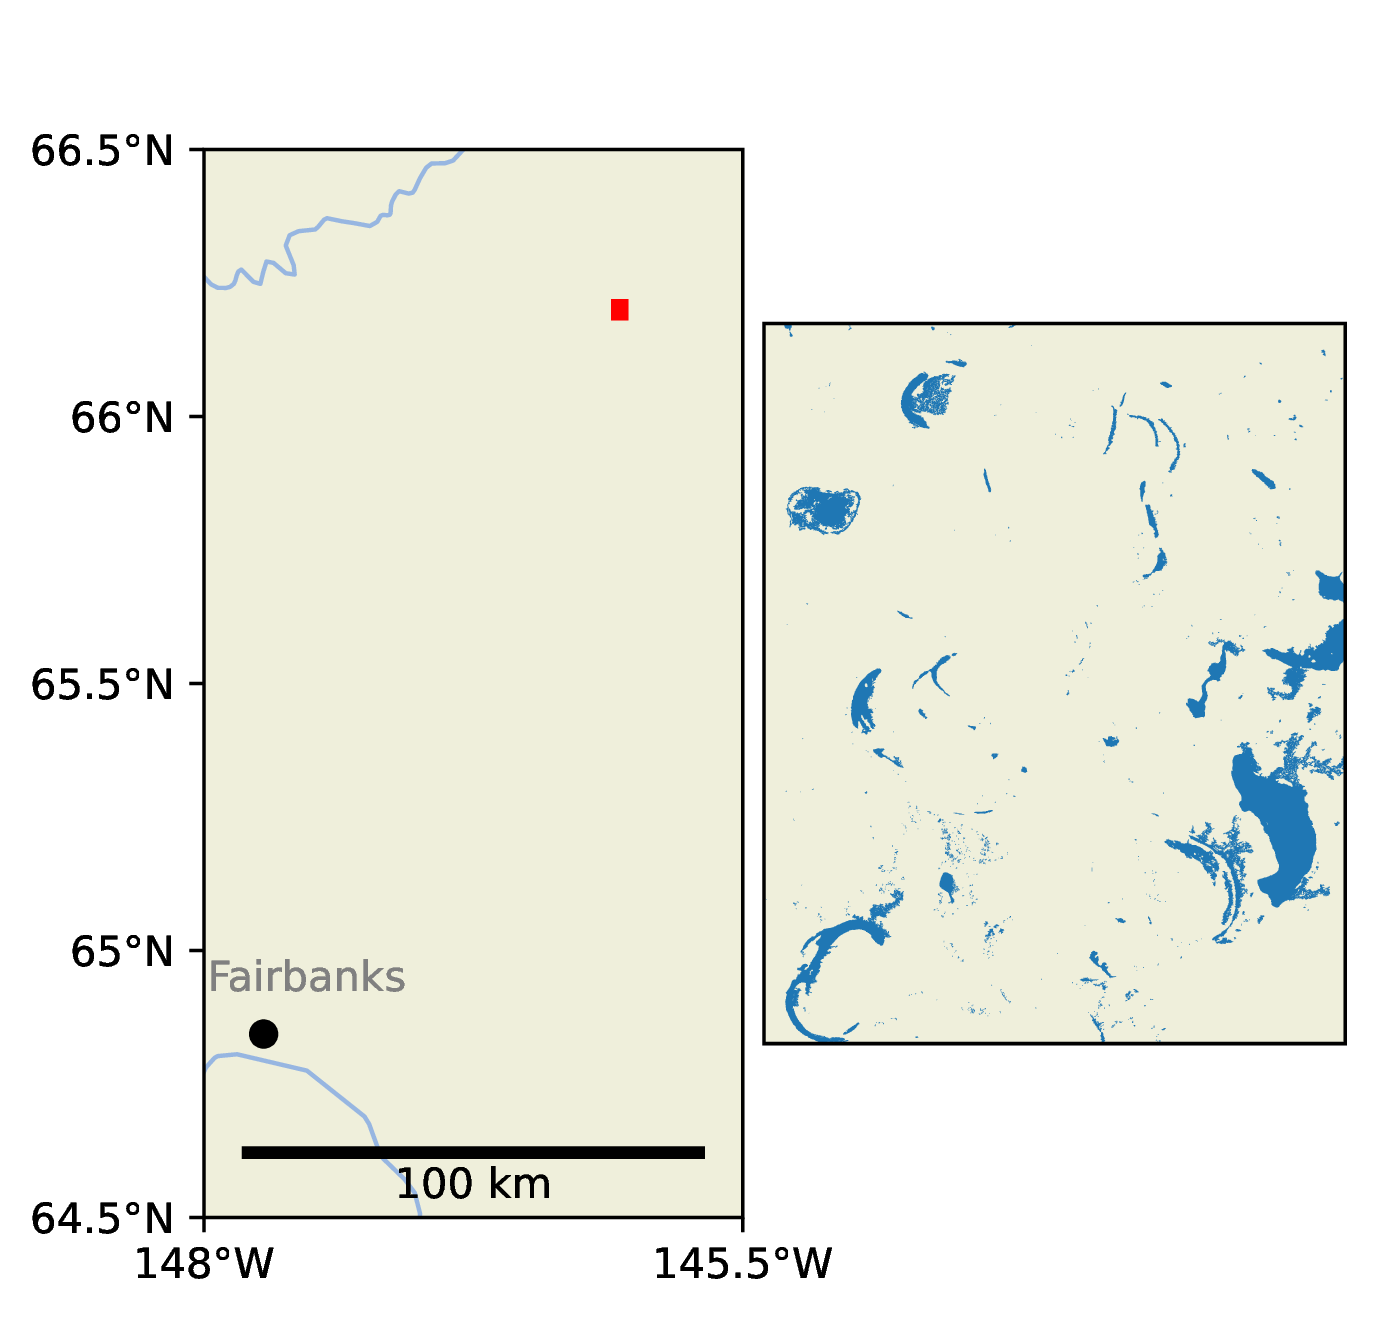
\includegraphics[width=9cm]{../figures/study_site}
	\caption{Map of our case study site centered northeast of Fairbanks at approximately 149 deg W, 66 deg N (left panel, red box) alongside a zoomed in view of our case study AOI with PeRL waterbodies (right panel).}
	\label{fig:study_site}
\end{figure}

\begin{figure}
	\centering
	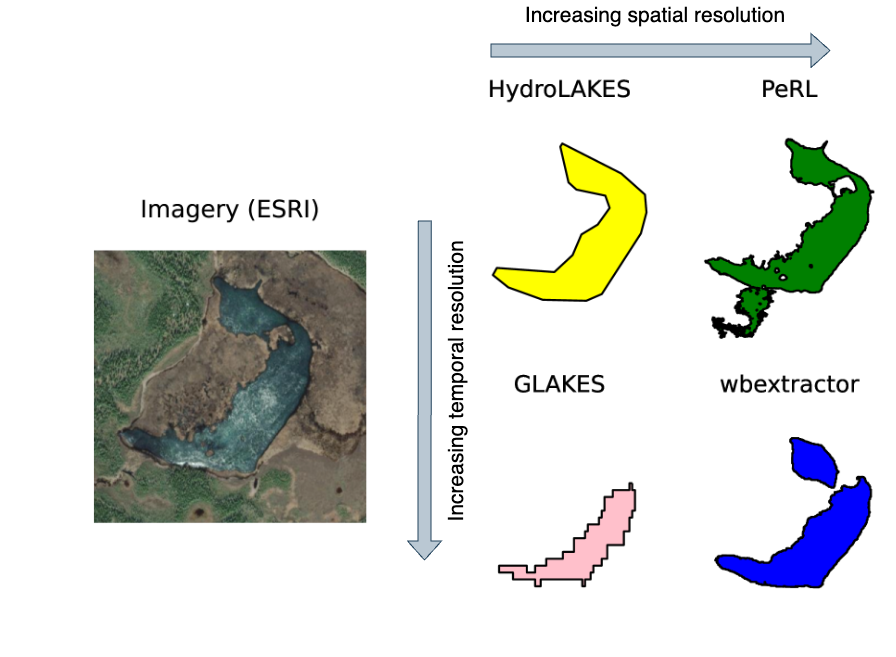
\includegraphics[width=12cm]{../figures/single_wb.drawio.png}
	\caption{A waterbody centered at approximately 146.03 deg W, 66.2 deg N. showing (left panel) imagery of the waterbody and a comparison (right panel) of various data products for the waterbody including at top left, the HydroLAKES data product which has the least amount of automated construction and the lowest spatial resolution. This contrasts with the output of our pipeline (wbextractor, bottom right), which produces a waterbody that is comparable to the manually delineated PeRL product but has a much more automated construction.}
	\label{fig:single_wb}
\end{figure}

\section{Results}

Images matching our quality criteria were available only from May-October due to seasonal snow and ice. Within the May-October time window, wbextractor retrieved 22 images in the time period of 2017-2022 (see Table S1 for a complete listing). The wbextractor tool identified 341 recurrent waterbodies from these images (within our AOI), using a specified recurrence threshold of 5\% which ranged in area from 1500 $m^2$ to 3.4 $km^2$. In Figure 4, we show a comparison between the overall distribution waterbodies identified by wbextractor (across all time steps) against that of other datasets. We found that the distribution of wbextractor waterbodies were a much closer match to the PeRL dataset (n=1181, 4 $m^2$ - 0.9 $km^2$) relative to the GLAKES (n=3, 6.5 x 104 $m^2$ - 0.17 $km^2$) and HydroLAKES (n=2, 1.4x105 $m^2$ - 0.25 $km^2$) datasets.

\begin{figure}
	\centering
	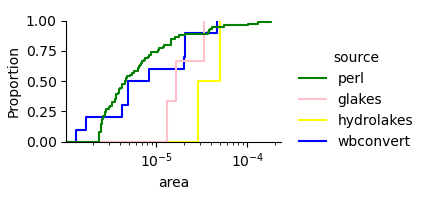
\includegraphics[width=10cm]{../figures/accuracy}
	\caption{Comparison of the Empirical Cumulative Distribution Function of waterbody area within each dataset used in the study (within our AOI). The output of the wbextractor tool (blue line) more closely matches the distribution waterbodies in the hand-delineated PeRL dataset (green line) relative to the other two products (pink and yellow lines).}
	\label{fig:accuracy}
\end{figure}

Beyond the similarity in terms of raw waterbody counts and area distributions, wbextractor and PeRL also share similarity in terms of the types of waterbodies they returned. Whereas GLAKES and HydroLAKES were missing all floodplain lakes, especially oxbow lakes, some of these were captured by the wbextractor tool (Figure 5). This ability to more accurately return floodplain lakes is a result of the trained TorchWBType model checkpoint we used in the pipeline which had a precision, recall, and F1 score of correct waterbody identification of 0.66, 0.70, and 0.68 respectively and misclassified only 22\% of waterbodies in the global ReaLSAT test set (119, n=540).

\begin{figure}
	\centering
	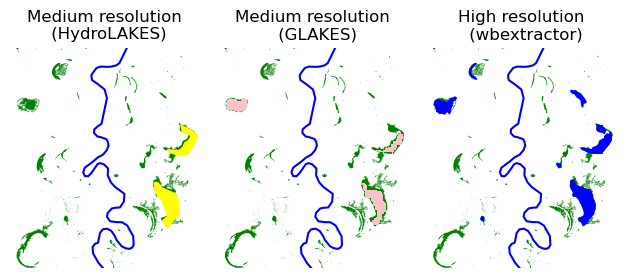
\includegraphics[width=11cm]{../figures/floodplain}
	\caption{Comparison between waterbodies in the manually-delineated PeRL dataset (green polygons) and those in the medium resolution HydroLAKES dataset (yellow polygons, left panel), the medium resolution GLAKES dataset (pink polygons, middle panel), and our wbextractor pipeline (blue polygons, right panel).}
	\label{fig:floodplain}
\end{figure}

Finally, our pipeline was able to track waterbody splitting and reforming as a result of flooding and/or drying. Note that wbextractor unlike the other datasets, can maintain a single waterbody identifier across multiple polygons when they have been joined at any prior or subsequent time step in the period of record (Figure 3). Overall, we found that only 54\% of waterbodies in the wbextractor dataset had a single configuration across all time steps. The remaining 46\% had at least one split/reform in the period of record with a mean split/reform count of 2.3 and a maximum split/reform count of 21 out of a possible 27 split/reform time steps.

\section{Discussion}

We found that our pipeline, which uses a combination of high resolution imagery together with modern web APIs and advanced ML algorithms, produced waterbody datasets with accuracy approaching that of labor-intensive manually delineated products. Furthermore, the high accuracy, low labor costs, and minimal computation overhead of the pipeline, provided the performance necessary to scale our approach to continental and global extents. Although the primary criteria for the design of our pipeline was accuracy and performance, we also built in features to maximize the flexibility with which the pipeline is configured and executed. From file formats, to imagery API choices, and image quality criteria, users are given the option to modify the default settings or substitute their own method for any step of the pipeline.

In our case study, we used a GeoTiff basemap to define our AOI but wbextractor also supports providing an AOI via vector file or numeric bounding box, which may be preferable, depending on the up/downstream application. Additionally, we used an extremely conservative set of quality flags to maximize pipeline performance (i.e. speed of execution) and accuracy, but these choices likely came at the cost of decreased sensitivity and comprehensiveness. Our aim with these quality flags was to maximize the exclusion of spurious waterbodies that may arise from inadequate accounting for cloud cover and or snow/ice and/or other imagery artifacts in order to focus on waterbody recurrence algorithm development. A potential benefit to a less stringent set of quality flags is that it would likely increase the number of time steps representing a given waterbody. This would provide greater temporal detail for downstream use as well as boost the ability of the recurrence algorithm to recover a greater number of ephemeral waterbodies in the output. The threshold at which a waterbody is considered recurrent (i.e. not ephemeral) is another area of flexibility afforded to users. In our case study, we attempted to compensate for our stringent image quality filters by using a low recurrence threshold of 5\% compared to more typical values near 10\% \citep{khandelwal2022realsat}. For downstream applications on long-time scales greater than a decade or so, it may be preferable to use a threshold higher than 10\% or some alternative strategy such as only retaining waterbodies that span the entire period of record without regard to the number of timesteps in which it is represented.

A key innovation of our pipeline is our inclusion of an ML waterbody classifier model for automated type identification and removal of spurious non-lake waterbodies. In our view, this is the missing piece for accurate scaling of time-resolved waterbody dataset creation to continental and global extents. This contrasts with prior approaches which consisted of either manual pruning of spurious waterbodies, wholesale removal of waterbodies in problematic regions/ecotypes (e.g. at high latitudes and in river-adjacent floodplains), or leaving spurious waterbody removal to the downstream user (sometimes without their knowledge). By default, the TorchWBType model only discriminates between lakes and non-lakes. Future improvements to the model should be aimed at increasing the number of classes in the model to more specifically target flooded agricultural fields (which are uniquely shaped and easily identified) as well as riverine floodplain lakes (e.g. oxbow lakes) and coastal embayments. Discrimination between wetlands and lake waterbodies would likely prove more difficult due to the challenges of automated wetland delineation from imagery and complexities associated with geoprocessing integrated lake, wetland, and stream datasets (Fergus et al. 2017). A related area of future research is in potential improvements to water discrimination algorithms. The wbextractor tool has the capability to “hook-in” a DeepWaterMap model checkpoint or a simple NDWI algorithm \citep{gaoNDWINormalizedDifference1996} within the pipeline but neither of these are specifically tailored to Planet imagery (Figure S1). This is an area where wider adoption of deep learning approaches such as U-Net would be extremely useful (e.g. \citet{mullenUsingHighResolution2023}).

We found that by incorporating high resolution imagery with advanced ML algorithms, we were able to produce a dataset approaching the accuracy of much more expensive hand-curated products. Although our pipeline does a better job of matching the number and area range of the lakes in the study area than GLAKES or HydroLAKES it still does not exactly match PeRL. This indicates that more development is needed to achieve this high standard of accuracy keeping in mind that our study was motivated by a hydrologic routing use-case, which in our experience would still benefit from the increased resolution and accuracy afforded by our tool even if it doesn't have as high of a resolution as manually delineated products. For hydrologic routing tasks, wbextractor is capable of resolving waterbodies to match the scale of the vector-river networks in which they are embedded. This has been recognized as a critical need in Earth System Model applications involving routing of streamflow and its constituents \citep{mizukamiVectorBasedRiver2021}. With the flexibility of our pipeline and the ability for automated type identification of pruning of spurious waterbodies, our tool has the potential to seed the next generation of hydrologic routing and watershed-centric research at the global scale particularly as it becomes more clear that static DEM-based products are inadequate in an era of rapid climate change.

\section{Data Availability Statement}

All data and code associated with this manuscript will be made available at: \href{https://doi.org}{https://doi.org}

\section{Acknowledgements}

J.Sta. built models, analyzed data, and wrote the paper. C.J.A. analyzed data. All authors reviewed and edited the paper. This work utilized data made available through the NASA Commercial Smallsat Data Acquisition (CSDA) Program. This work was supported by Los Alamos National Laboratory (LDRD-20210213ER, LDRD-20220697PRD1, LDRD-20230701DI).

\bibliographystyle{jsta}
\bibliography{hydroml_2023}

\end{document}
